\documentclass[final]{article}


\usepackage[final,main]{aps360}
\usepackage[utf8]{inputenc} % allow utf-8 input
\usepackage[T1]{fontenc}    % use 8-bit T1 fonts
\usepackage{hyperref}       % hyperlinks
\usepackage{url}            % simple URL typesetting
\usepackage{booktabs}       % professional-quality tables
\usepackage{amsfonts}       % blackboard math symbols
\usepackage{nicefrac}       % compact symbols for 1/2, etc.
\usepackage{microtype}      % microtypography
\usepackage{xcolor}         % colors
\usepackage{tikz}           % native vector figure
\usetikzlibrary{arrows.meta,positioning}

\title{Robust Cross-Day Hand-Gesture Recognition from Wrist Surface\\
Electromyography Signals Using a 1D Convolutional Neural Network}

\author{%
  Grace MacLeod \\
  \url{https://github.com/gracemacleodd/APS360-EMG-Gesture-Recognition}
}

\begin{document}

\maketitle

\vspace{-0.55in}

\section*{Introduction}
Surface electromyography (sEMG) records the electrical activity of contracting muscles and is a leading signal for wearable human--computer interfaces, prosthetic control, and rehabilitation devices because it can reveal an intended hand gesture with little or no overt movement. The main obstacle to deployment is \emph{cross-day} (cross-session) degradation: a model trained on one day loses substantial accuracy on another because electrode placement shifts, skin impedance changes, and muscle state vary between sessions. This project develops and evaluates a one-dimensional convolutional neural network (1D CNN) that classifies static hand gestures from multichannel \emph{wrist} sEMG and explicitly measures how much accuracy is lost across days. The goal is to maximize multiclass gesture accuracy while minimizing this cross-day gap; we target the wrist because a wrist-worn band is the most practical wearable form factor. Deep learning suits this task: sEMG gestures are high-dimensional, non-stationary, multichannel time series whose features are hard to hand-engineer, and a 1D CNN learns temporal and inter-channel structure directly from raw windows, repeatedly outperforming hand-crafted-feature pipelines for sEMG \citep{atzori2016deep,coteallard2019transfer}. The pipeline is also a reusable testbed for later electrode-hardware comparisons (e.g., flexible or MXene-based electrodes), which are outside this project's scope.

\section*{Illustration}
Figure~\ref{fig:pipeline} summarizes the pipeline and the central cross-day evaluation.

\begin{figure}[!h]
  \centering
  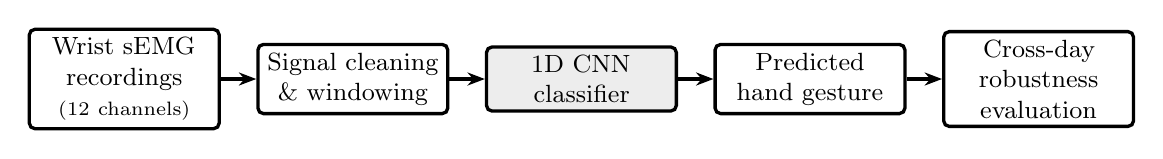
\begin{tikzpicture}[
      node distance=4.5mm,
      box/.style={rectangle, rounded corners=2pt, draw=black, very thick,
                  align=center, inner sep=3pt, minimum height=8mm, font=\small,
                  text width=22mm},
      cnn/.style={rectangle, rounded corners=2pt, draw=black, very thick,
                  fill=black!7, align=center, inner sep=3pt, minimum height=8mm,
                  font=\small, text width=22mm},
      arr/.style={-{Stealth[length=2.2mm]}, very thick}
    ]
    \node[box] (raw) {Wrist sEMG recordings\\\scriptsize(12 channels)};
    \node[box, right=of raw] (proc) {Signal cleaning \& windowing};
    \node[cnn, right=of proc] (cnn) {1D CNN classifier};
    \node[box, right=of cnn] (pred) {Predicted hand gesture};
    \node[box, right=of pred] (eval) {Cross-day robustness evaluation};
    \draw[arr] (raw) -- (proc);
    \draw[arr] (proc) -- (cnn);
    \draw[arr] (cnn) -- (pred);
    \draw[arr] (pred) -- (eval);
  \end{tikzpicture}
  \caption{Proposed pipeline: cleaned, windowed wrist sEMG is classified by a 1D CNN; same-day vs.\ held-out-day accuracy quantifies cross-day robustness.}
  \label{fig:pipeline}
\end{figure}

\section*{Background \& Related Work}
The \textbf{GRABMyo} dataset \citep{pradhan2022grabmyo,jiang2022grabmyophysionet} provides forearm and wrist sEMG from 43 participants recorded on three separated days (Days 1, 8, and 29) while performing 16 static hand and finger gestures at 2048\,Hz; it is purpose-built for multi-day robustness and is the dataset used here. \citet{atzori2016deep} showed CNNs on raw sEMG windows match or exceed hand-crafted-feature classifiers, motivating our learned-feature approach. \citet{coteallard2019transfer} tackled the closely related cross-session problem with transfer learning across users and sessions to counter non-stationary sEMG, directly informing our cross-day framing. \citet{geng2016instantaneous} achieved high gesture accuracy from high-density sEMG with deep CNNs, evidence that such models capture discriminative sEMG structure. The \textbf{Ninapro} dataset \citep{atzori2014ninapro} established a widely used sEMG benchmark and the evaluation conventions we adopt. Across these works, learned convolutional features are effective for sEMG, yet cross-day generalization remains the open challenge this project targets.

\section*{Data Processing}
\textbf{Source.} We use the open-access GRABMyo dataset \citep{pradhan2022grabmyo,jiang2022grabmyophysionet} (PhysioNet), restricted to the \emph{wrist} band: 12 monopolar channels (two rings of six electrodes) at 2048\,Hz over three days. \textbf{Organization.} Recordings are indexed by participant, session/day, gesture, and trial (the dataset's per-session/per-participant folders), so each window is traceable to its day and trial. \textbf{Cleaning.} Each channel is band-pass filtered (20--450\,Hz) with a 60\,Hz notch to suppress motion and line noise, then re-referenced by the common-average procedure across the wrist ring; trials with saturated, flat, or missing segments are flagged, excluded, and logged. \textbf{Windowing.} Signals are segmented into 200\,ms windows with 50\% overlap (common sEMG practice); at 2048\,Hz each window is a $12\times410$ array. \textbf{Normalization and tensors.} Per-channel mean and standard deviation are computed on \emph{training} windows only and applied unchanged to validation and test windows, stored as PyTorch tensors of shape $(N,12,410)$ with integer labels. \textbf{Splits and leakage control.} Splitting is done at the trial/day level \emph{before} windowing, so overlapping windows from one 5\,s contraction never span two splits. (i)~\emph{Same-day split:} within each day, gesture trials are partitioned into train/validation/test (e.g., five/one/one trials), an optimistic within-session reference. (ii)~\emph{Cross-day split:} the model trains on Days~1 and~8 and tests on the held-out Day~29 (validation drawn from the training days), reproducing a user re-donning the band on a later day. Both are evaluated per subject and averaged. \textbf{Evaluation.} We report overall accuracy, macro-averaged F1 (robust to class imbalance), and a confusion matrix; the headline metric is the \emph{cross-day drop}, same-day minus cross-day accuracy, which the project aims to shrink.

\section*{Architecture}
The main model is a 1D CNN taking the $12\times410$ window (channels as features, time as the convolution axis). A preliminary design stacks two to three convolutional blocks, each a 1D convolution (kernel $\approx$5, increasing filters such as 32/64/128), batch normalization, ReLU, and max pooling; a dropout layer ($\approx$0.3--0.5) then precedes a global average pooling layer, one or two fully connected layers, and a softmax over the 16 gesture classes. Training uses cross-entropy loss with Adam and early stopping on validation macro-F1. Exact layer counts and hyperparameters will be tuned on validation; a CNN--LSTM variant is a possible extension once the 1D CNN works.

\section*{Baseline Model}
The baseline is a support vector machine (SVM) with an RBF kernel trained on classical time-domain features: for each window and each of the 12 channels we extract root mean square, mean absolute value, waveform length, and zero crossings (the Hudgins set), giving a $4\times12=48$-dimensional vector standardized with training statistics. It is implemented in scikit-learn with the regularization parameter $C$ and kernel width $\gamma$ tuned on validation, using the same windows and splits as the CNN. Comparing the two under both conditions tests whether learned features beat engineered ones and degrade less across days.

\section*{Ethical Considerations}
Performance may vary across individuals because of physiological differences, electrode placement, skin condition, and recording setup, so accuracy on this dataset may not transfer to a new user. The GRABMyo participants are a small group of healthy adults aged roughly 24--35; results may not represent children, older adults, people with neuromuscular conditions, or noisy real-world settings, and should not be generalized beyond this group. In an assistive or prosthetic device, misclassified gestures could cause unintended, unsafe actions, so the system must be treated as a research prototype, \emph{not} a clinically validated tool. Data are used under the dataset's PhysioNet license and intended-use terms, participants are not re-identified, and any released code and weights will carry the same cautions.

\newpage
\bibliographystyle{plainnat}
\bibliography{references}

\end{document}
